

\section{Discussion}





\subsection{Explaining Traversal Variations in Chemistry}

Increasing DSi concentration with decreasing elevation suggests the springs are sampling increasingly longer flow paths. This is because longer flow paths allow for more water-rock interaction, which scavenges more Si from the silicate rocks. While most traverses show such a trend, this does not happen in Traverse 1. There are several possible reasons for this. For one, the lowermost springs are likely to be close to the Melamchi river which is more dilute than the most concentrated springs in the traverse. It is unlikely that the decrease is caused by a dilution effect at the start of the monsoon such as that show in Figure (ref). This is because these DSi trends are consistent across multiple seasons within error. Clearly, however, samples collected in September will be relatively more dilute than those collected in April.

\bsk

A decrease in Si at lower elevations here could also suggest precipitation of secondary minerals. Linear trends in plot (b?) for Traverses 1, 3, and 5 show an increase in Na/Si as elevation decreases. Si is involved in the backward secondary mineral precipitation weathering reaction, and Na is not, as evidenced in equation (?). In other words, elevated Na/Si is interpreted as a sign of a closer approach to equilibrium, as more Si is scavenged from the water to form secondary precipitates, while the Na is only involved in dissolution. This is consistent with the Traverse 1 springs having the highest concentrations of Si in the catchment as chemical equilibrium is approached. 

\bsk

Plots of Na/Si against elevation coloured by season can also be used to infer how consistently a given flow path is sampled. Because Na/Si is primarily controlled by the balance of dissolution and reprecipitation, and therefore the average age of water in the flow path, consistency of this value over time points to the same flow path length being sampled for a given rate of reaction. Under the steady state assumption assumption $\partial C/\partial t = 0$ used in the residence time models, the Na/Si ratio should be constant over time at a given elevation if the same flow path is sampled. For both Traverse 3 and 5, the Na/Si ratio against elevation does not change between different seasons. However, there is a better correlation in Traverse 3 which suggests the flow paths here are more consistently sampled.

\bsk

The consistency with which flow paths are sampled in Traverse 3 is more apparent when plotting Na/Si in one season against the rest (note that Figure \ref{fig:spatial_changes_spring8} the Na/Si values are uncorrected to showcase results collected in more than two seasons). 

\begin{figure}[h]
    \centering
    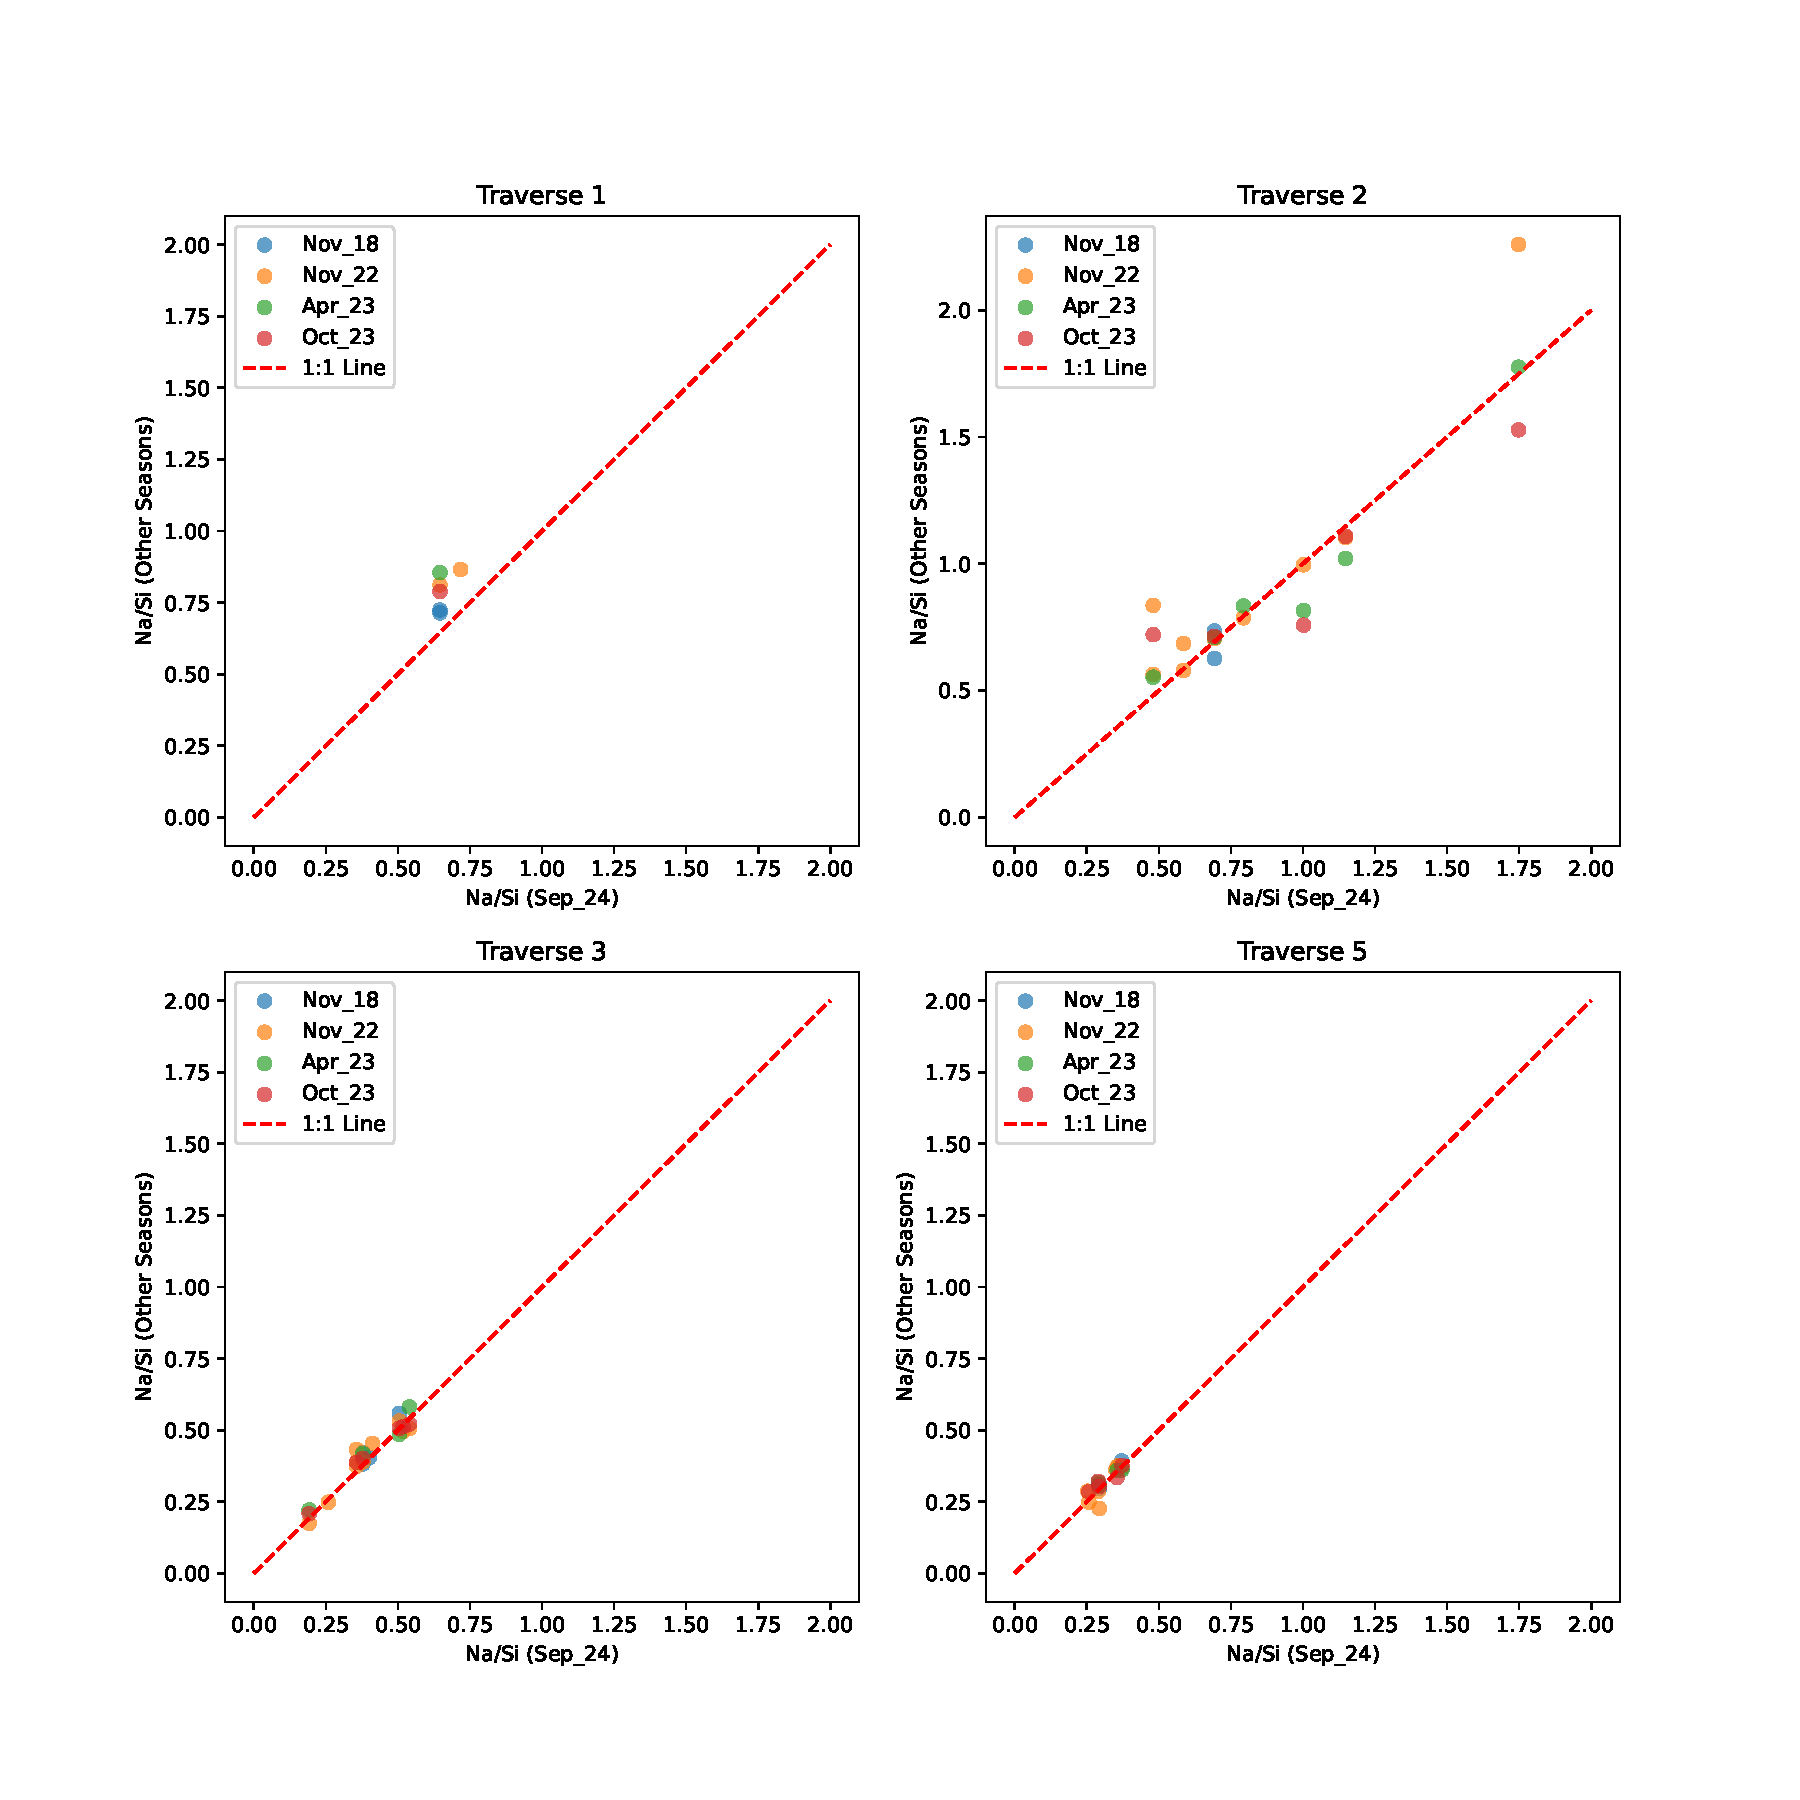
\includegraphics[width=\textwidth]{Na_Si_Seasons.pdf}
    \caption{How Na/Si varies for different traverses. Traverse 4 is not plotted due to the lack of samples.}
    \label{fig:spatial_changes_spring8}
\end{figure}
\FloatBarrier

The scatter in these plots reflect temporal variability in the spring chemistry. Traverses 1 and 5 both display tight scatter, consistent with the notion that the flow paths here are consistently sampled. More notable here are the differences in Na/Si values between traverses. These how the spatial variability between traverses is more significant than the temporal variability. It is possible, and quite likely that all traverses flow paths are connected one to the other. When investigating model differences, however, a knowledge of which traverse accounts for what discrepancy allows for the contribution of spatial variation toward the overall interpretation to be taken into account.









\subsection{Strontium Isotopes suggest Little Rainwater Influence}

Radiogenic strontium isotope analyses of springs show significant variation between different traverses. Due to the unique source-tracking nature of strontium isotopes, this is potentially explained with varying lithology (see Appendix / ref). In other words, different traverses sample lithologies that have different strontium isotopic composition, and the water chemistry reflects this. These variations are within the range of Higher Himalayan Crystalline Series (HHCS) rocks found in the region (Tipper et al., 2006). It is unlikely that the source of the Sr isotopes is from the Lesser Himalayan Series (LHS) rocks. Indeed the Main Central Thrust (MCT) is several km south of Melamchi.

\bsk

Sr isotope values of rain are consistent with the expected values for rainwater, with the exception of those sampled at low elevation (Galy, France-Lenord, Derry, 1999). The lowest Sr isotope value for rain is very close to the reported value for seawater, which is 0.70917. These rain samples with low strontium isotopic composition therefore likely reflect seawater strontium isotope values, indicating little contamination from dust or particles. The uncontaminated samples are indeed found at the higher elevations, and they show low chloride concentrations consistent with rain.

\bsk

Strontium isotope ratios used alongside strontium concentrations can be used to determine mixing between different endmembers (Faure, 1986; See Appendix). Plots of $\ddfrac{^{87}Sr}{^{86}Sr}$ against $\ddfrac{1}{Sr}$ that yield straight lines are indicative of mixing trends. 

\begin{figure}[p]
    \centering
    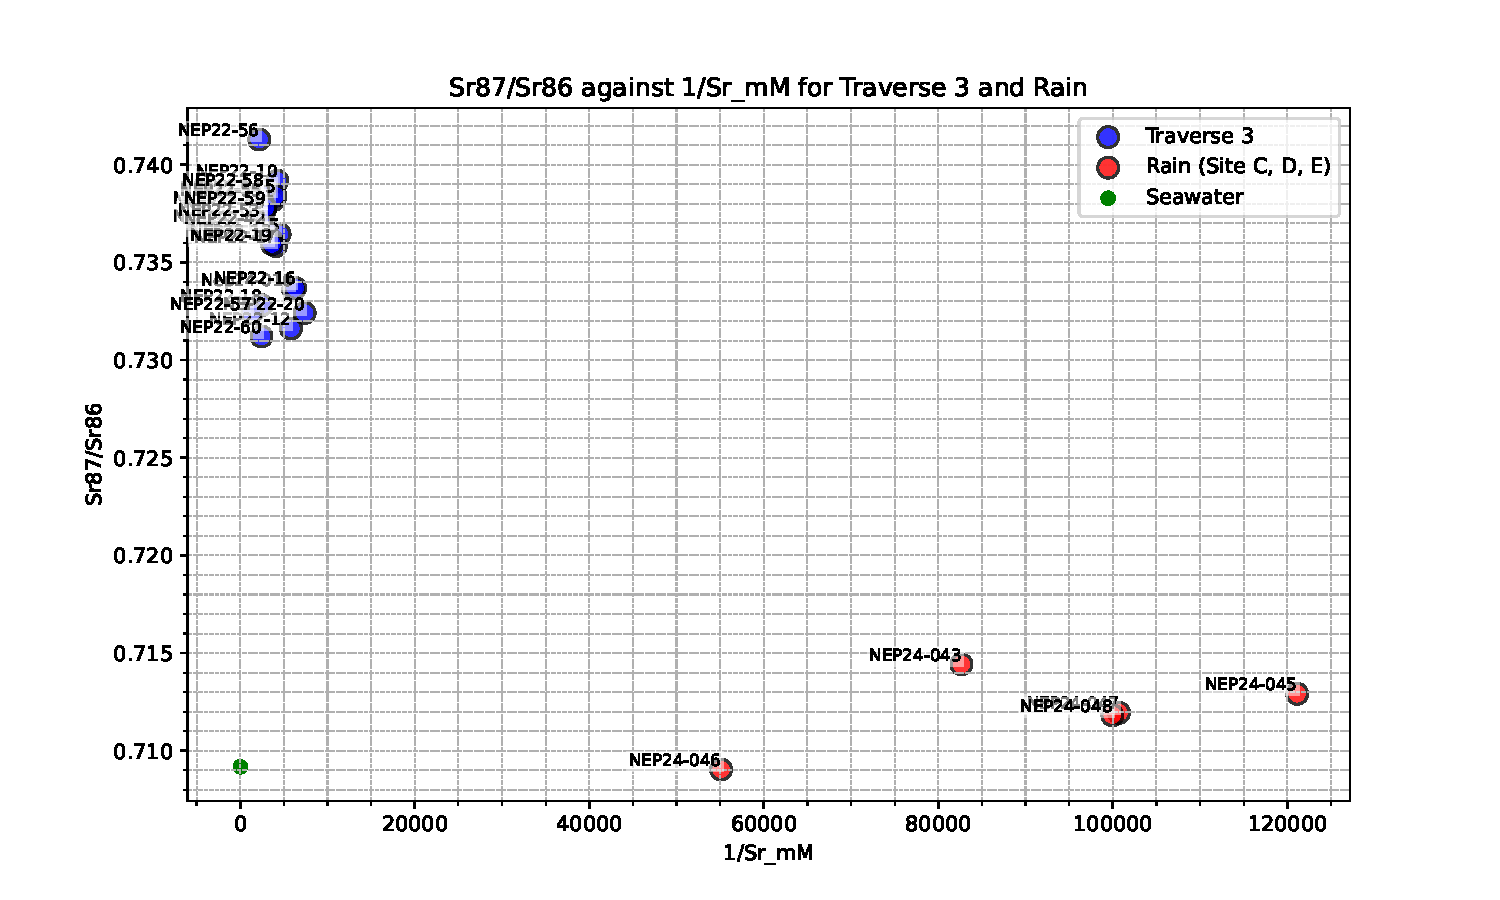
\includegraphics[width=\textwidth]{Sr87_Sr86_1Sr_Rain.pdf}
    \caption{Strontium isotope differences display difference in lithology tapped in. Cite Quade and Tipper papers; Rain analysed for Sr isotopes and Cl. Something about contamination lower down; How samples of Traverse 3 compare to the rain samples}
    \label{fig:discussion3}
\end{figure}

\FloatBarrier

Figure \ref{fig:discussion3}a shows $\ddfrac{^{87}Sr}{^{86}Sr}$ against $\ddfrac{1}{Sr}$ for springs and rain in the catchment. Comparing spring samples to the rain [Change graph], it is clear that the latter does not exert a significant control on the spring chemistry, not even for the presumably shortest flow paths at the top of the ridge. In other words, chemical weathering reactions are likely to be the main control on the spring chemistry.













\subsection{Model Constraints on Residence Time}

Residence times in Traverse 1 are explainably the longest in the catchment. The springs here at are the lowest elevation, so the flow paths are presumably the longest. This is consistent with the highest DSi concentration of the catchment, and evidence for secondary precipitation of kaolinite at the lowest elevations (See Figure ?b). In Traverse 1, the Fontorbe model predicts a peak of $\approx$ 100 years, while the Maher model has a much higher residence time of $\approx$ 600 years. The discrepancy is likely due to how the models are formulated.

\begin{table}[h]
    \centering
    \renewcommand{\arraystretch}{2.2} % Adjust row spacing
    \begin{tabular}{cc}
        \toprule
        \textbf{Fontorbe} & \textbf{Maher} \\
        \midrule
        $\displaystyle T_f  = \frac{\left(C_h - C_o\right)\cdot\phi}{\left(1-f\right)\cdot R_n}$ & 
        $\displaystyle T_f = \frac{C_{eq} \cdot \left(C - C_0\right)}{e^2 R_n \left( C_{\text{eq}} - C \right)}$ \\ [10pt]
        % $\displaystyle R_n  = \frac{\left(C_h - C_o\right)\cdot\phi}{\left(1-f\right)\cdot T_f}$ & 
        % $\displaystyle R_n = \frac{C_{eq} \cdot \left(C - C_0\right)}{e^2 T_f \left( C_{\text{eq}} - C \right)}$ \\
        \bottomrule
    \end{tabular}
    \caption{Comparison of equations from Fontorbe and Maher}
    \label{tab:equations}
\end{table}

The difference in the models comes from the equilibrium concentration in the Maher formula. Indeed, for this study's formulation, the equilibrium concentration is taken to be the highest in the catchment, 869 $\mu$M DSi. This concentration corresponds to a spring in Traverse 1. Note that in the Maher and Chamberlain (2013) model setup, an equilibrium concentration of 375$\mu$M DSi is chosen from the global river data of Gaillardet et al. (1999). This makes sense for a theoretical model but is clearly not appropriate for this catchment. The Fontorbe model, on the other hand, does not depend on the equilibrium concentration. The $\frac{C_{eq}}{(C_{eq} - C)}$ term in the Maher model gets larger as the concentration approaches equilibrium. As a result of this, the Maher model consistently predicts longer residence times than the Fontorbe Model at higher DSi concentrations, while the opposite is true at lower DSi concentrations. It also follows that for Traverse 1 the $\frac{C_{eq}}{(C_eq - C)}$ term grows arbitrarily large, hence the strong discrepancy found in Figure (?c).

\bsk

The formulation is different because of how the two models approach rate of reaction. This is constant in the Fontorbe model, and depends on the equilibrium concentration for the Maher model (see Eqn ?). Indeed, as equilibrium concentration is reached in the Maher model, the reaction rate will decrease, and the residence time will increase. It is unrealistic that reaction rate continue to be constant as the reaction progresses, and so the Maher model more accurately reflects water that is close to equilibrium.

\begin{figure}[h]
    \centering
    \includegraphics[width=0.8\textwidth]{TheoreticalCeq.pdf}
    \caption{Comparison of how concentration changes with flow path length for the two models, and different equilibrium concentration}
    \label{fig:discussion8}
\end{figure}

\FloatBarrier

There is an argument to be made as to whether it is appropriate to choose the highest DSi concentration in the catchment as the equilibrium concentration. Maher (2011) details several ways in which the Maher model concentrations could change depending on the conditions. For example, increasing PCO$_2$ would increase the concentration of DSi at equilibrium. This aspect of the testing undergone in this study is therefore not well constrained. A more pressing concern, however, is whether the springwaters sampled are actually close to equilibrium. The free energy of reaction can be used to determine this.


In this way it is plausible that ~10 years could be how long the water is spending in the catchment, consistent with the \textcolor{red}{both} models. Such a finding suggests that the delay in river discharge of Andermann et al. (2013) is likely only recording surface or near-surface flow. The shorter flow paths here could plausibly be associated to residence times of a few months. 





\subsection{Free Energy Calculations}

A further constraint on the approach to equilibrium of a water packet is the free energy of reaction, which can be calculated using the activity of the ions in solution. Free energy is defined as:\textcolor{red}{cite}

\begin{equation}
    \Delta G = \Delta G^0 + RT \ln Q
\end{equation}

The plagioclase to kaolinite reaction is given by equation \ref{eq:10}. The parameters for the standard free energy of reaction are calculated using the pygcc python package (cite). The package gives the standard properties of solid-solution species and reactions, such that $\Delta G^0$ can be calculated:

\begin{equation}
    \Delta G^0 = \Delta G^0_{products} - \Delta G^0_{reactants} = -RT \ln K
\end{equation}\\
K is calculated using the database obtained from pygcc using The Geochemist's Workbench® Rxn program(ref). Q is calculated as the ion activity product of the reaction, assuming an ideal system whereby the activity is equal to the concentration of the ion in the water \textcolor{red}{Assuming the activities of the solid phases plagioclase and kaolinite are 1, the activity of water is 1, and the activity of the ions in solution are equal to their concentration, the free energy of reaction can be calculated. }

\begin{equation}
    Q = \frac{a_{\mathrm{Kaol}}^{0.6}\,a_{\mathrm{Na}^{+}}^{0.8}\,a_{\mathrm{Ca}^{2+}}^{0.2}\,a_{\mathrm{SiO_{2}(aq)}}^{1.6}}
           {a_{\mathrm{An_{20}}}\,a_{\mathrm{H}^{+}}^{1.2}}
\end{equation}\\

It is important to note that the composition of the plagioclase is important. The free energy of reaction is lowered by the presence of a solid solution between albite and anorthite (Dubacq, 2022). \textcolor{red}{In our case...}

\newpage

\textcolor{red}{Need to write }
\begin{figure}[H]
    \centering
    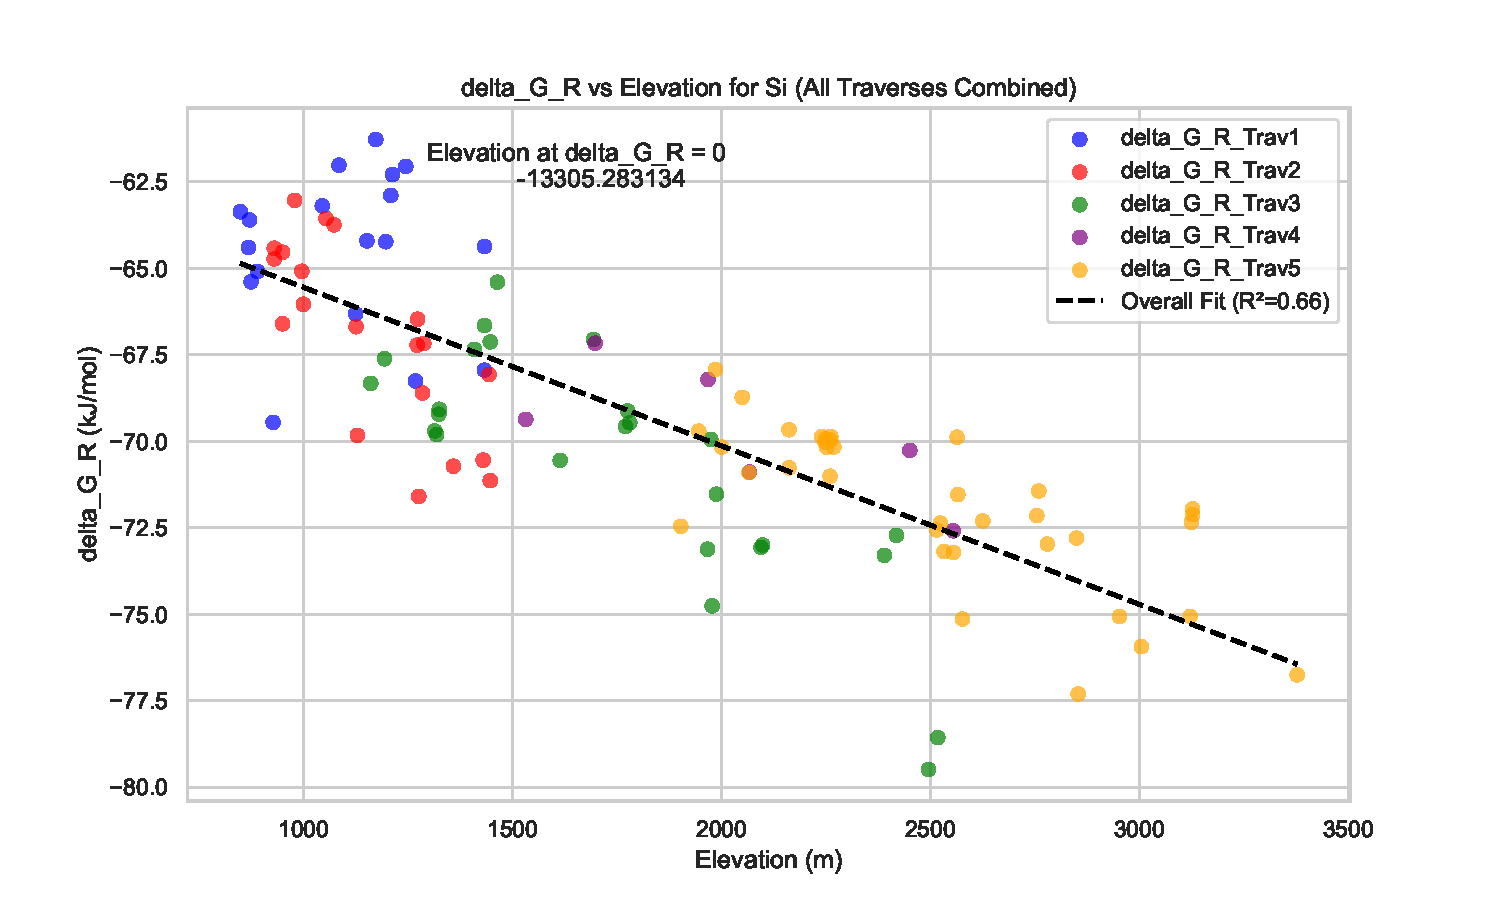
\includegraphics[width=0.9\textwidth]{delta_G_R_Si_combined_fit.pdf}
    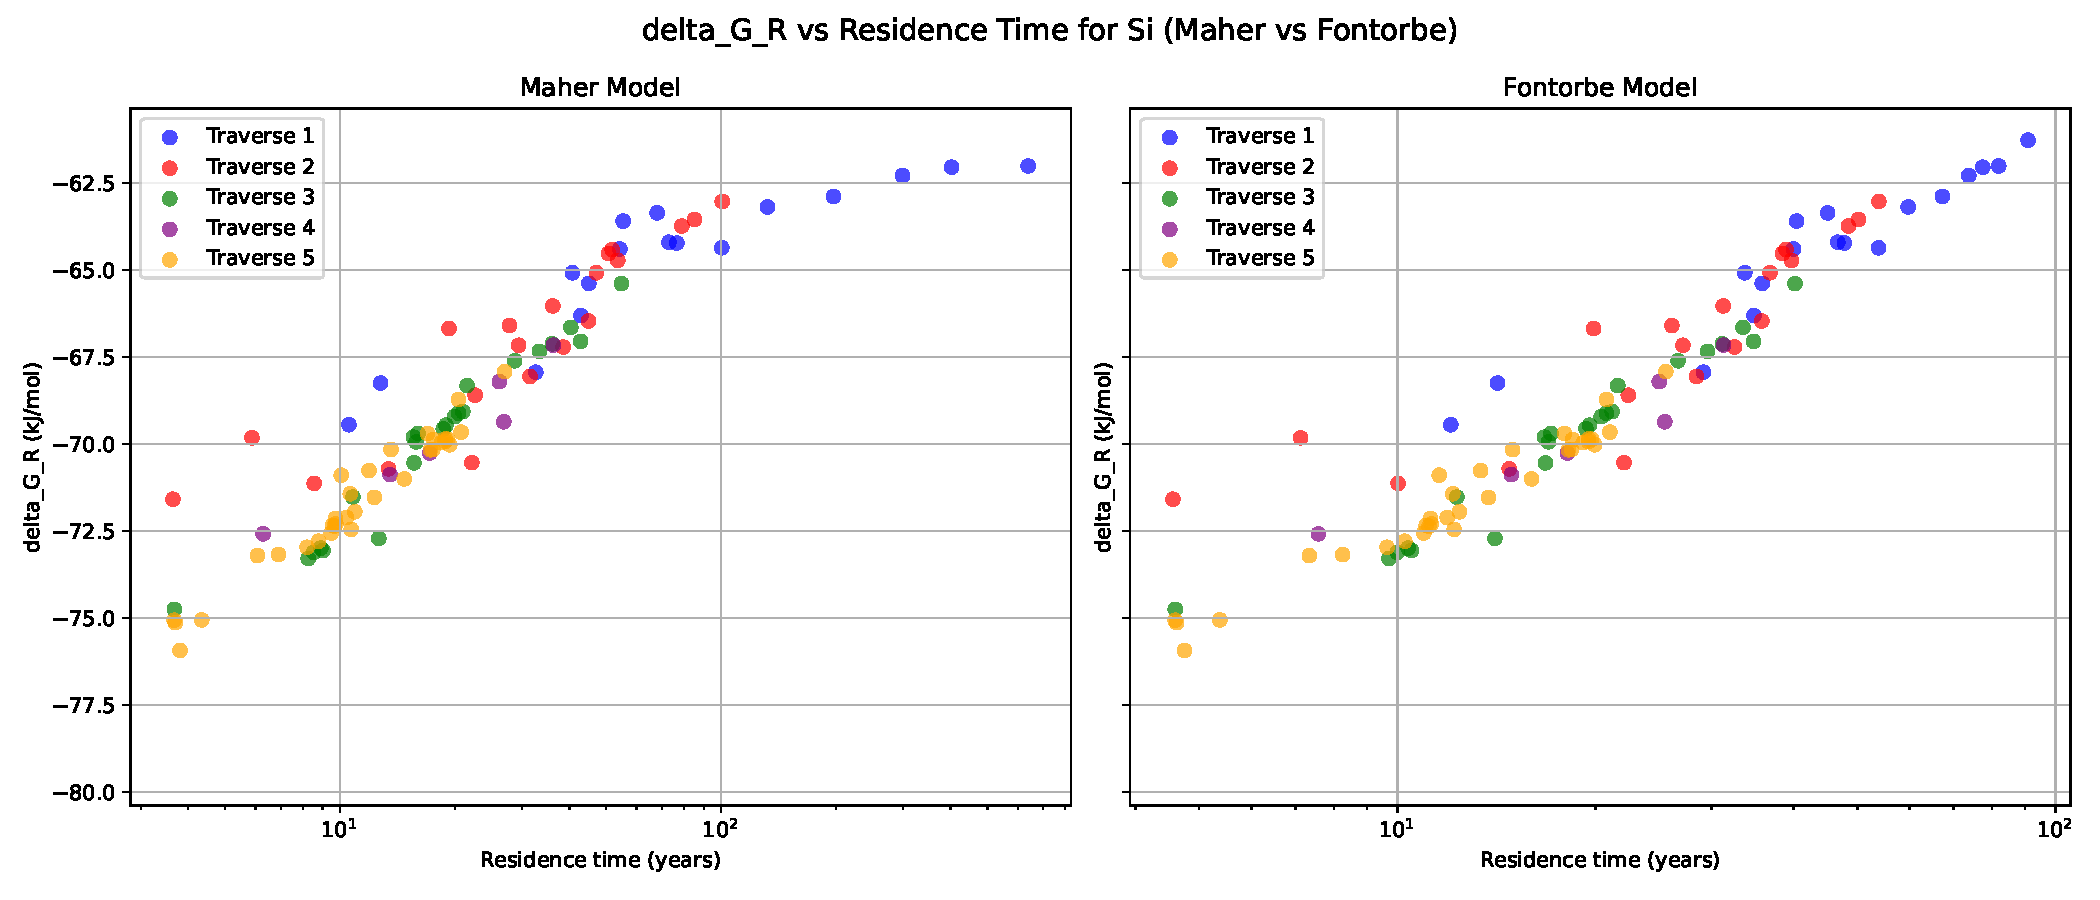
\includegraphics[width=0.9\textwidth]{delta_G_R_Si_time_Maher_vs_Fontorbe.pdf}
    \caption{Comparison of the delta G obtained against elevation. Comparison of delta G with residence time for both models}
    \label{fig:discussion8}
\end{figure}

\FloatBarrier


\newpage

\subsubsection*{Constraints on Reaction Rate}

Figure \ref{fig:discussion8} shows a decrease in $\Delta G$ as elevation decreases for all traverses, consistent with water getting closer to equilibrium as the flow path length increases. However, the free energy is only on the order of -60 kJ/mol at the longest flow path. This is not close to the -10kJ/mol that Kampman et al. (2014) suggest is the "near equilibrium plateau". Especially for Traverse 1, this suggests that the $C_{eq}$ chosen for the Maher model is not appropriate. In order for the Maher model to be accurate in its estimation of residence time and rate of reaction as equilibrium is approached, given the trend in $\Delta G$, the equilibrium concentration should be much higher than 869 $\mu$M DSi, on the order of five times as much.

\bsk

There might be an argument, also, to suggest that the reaction rate is not as high as the models suggest. Indeed, at those values, laboratory rates might be more appropriate \textcolor{red}{Have the Kampman table? Lab rates of reaction are much faster for this }. One sure test is to compare the free energy obtained for the samples in Traverse 3 to those in Traverse 1. Given that the equilibrium concentration for the residence time is taken from this latter traverse (see Figure in results, ref), according to the formulation of the Maher model this should be closest to equilibrium.

\bsk
 Hence, it is likely that a larger reaction rate is needed to characterise these groundwaters. This has implications for the residence times calculated using these models, as the former and latter are inversely proportional.


\textcolor{red}{Bit about Maher assuming equilibrium reached -> Maher not correct to implement here. Also mike permeability sketch???}


\begin{figure}[h]
    \centering
    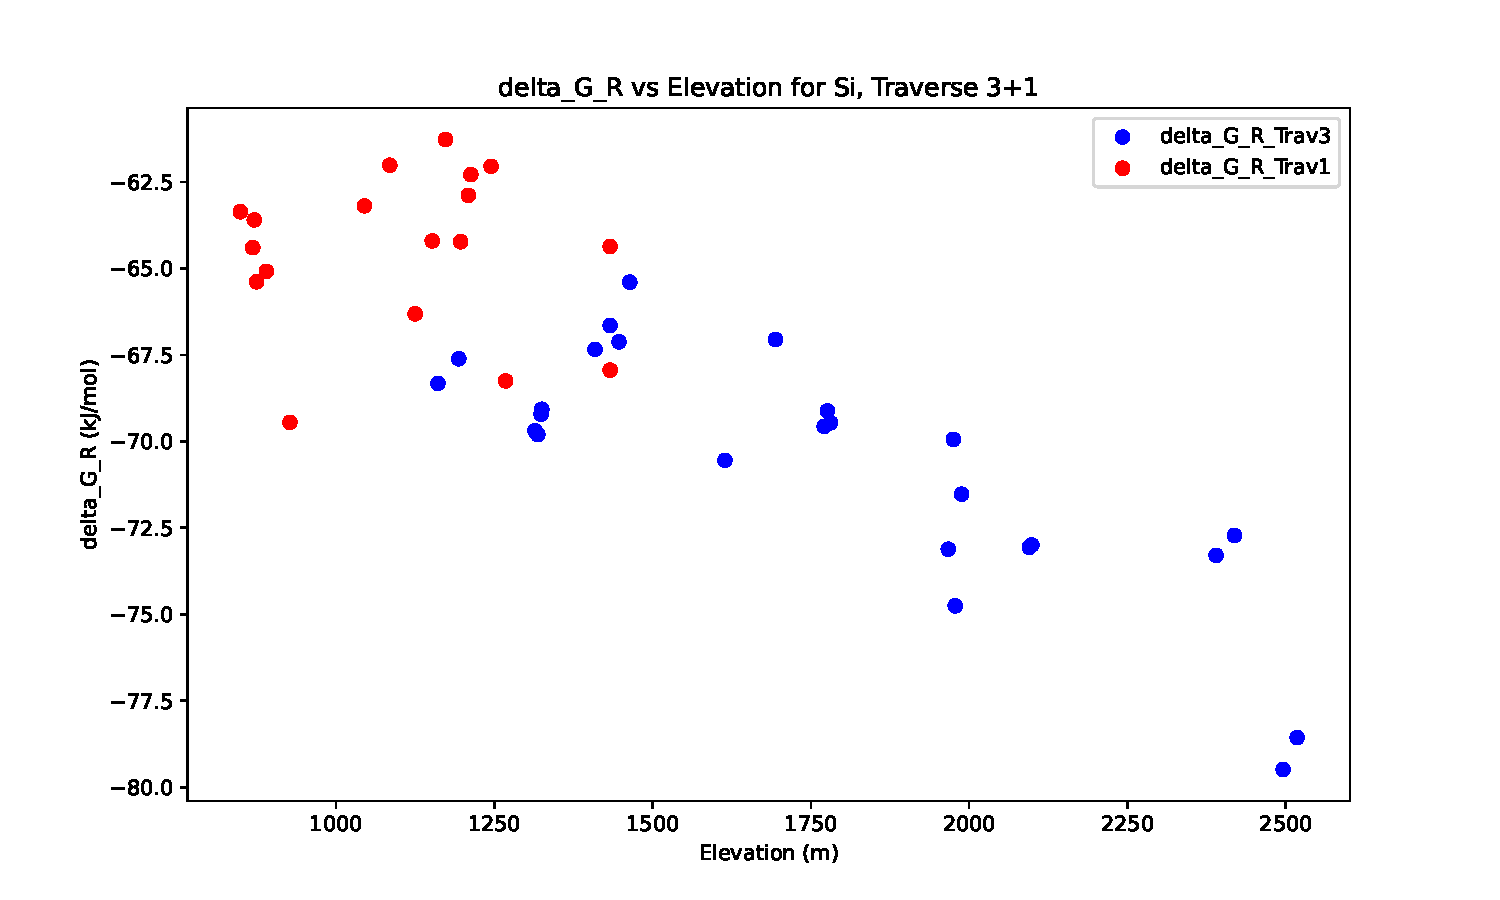
\includegraphics[width=\textwidth]{delta_G_R_Si_comparison_Trav1.pdf}
    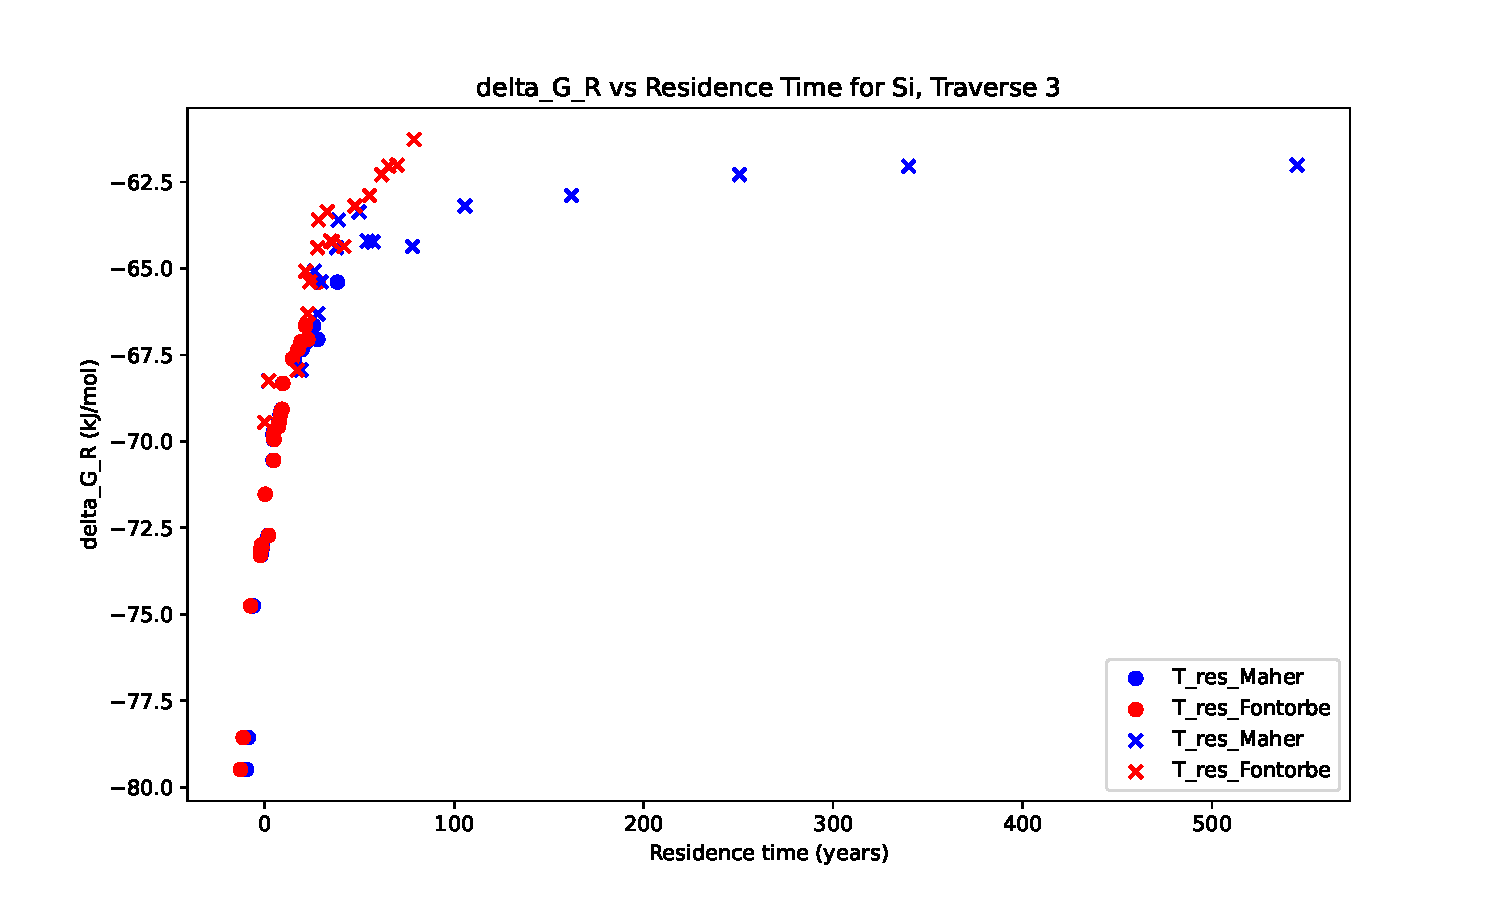
\includegraphics[width=\textwidth]{delta_G_R_Si_time_trav1.pdf}
    \caption{Comparison of the delta G obtained against elevation for Traverse 1 and Traverse 3. And residence time comparison, Note how Maher predicts really high residence times when Ceq is approached}
    \label{fig:discussion9}
\end{figure}

\FloatBarrier







REMEBER TO MENTION ANDERMANNN